\documentclass{article}
\usepackage[margin=1in]{geometry}
\usepackage{graphicx}
\usepackage{float}
\begin{document}
\section*{S7.3(B)}
\begin{figure}[H]
\centering
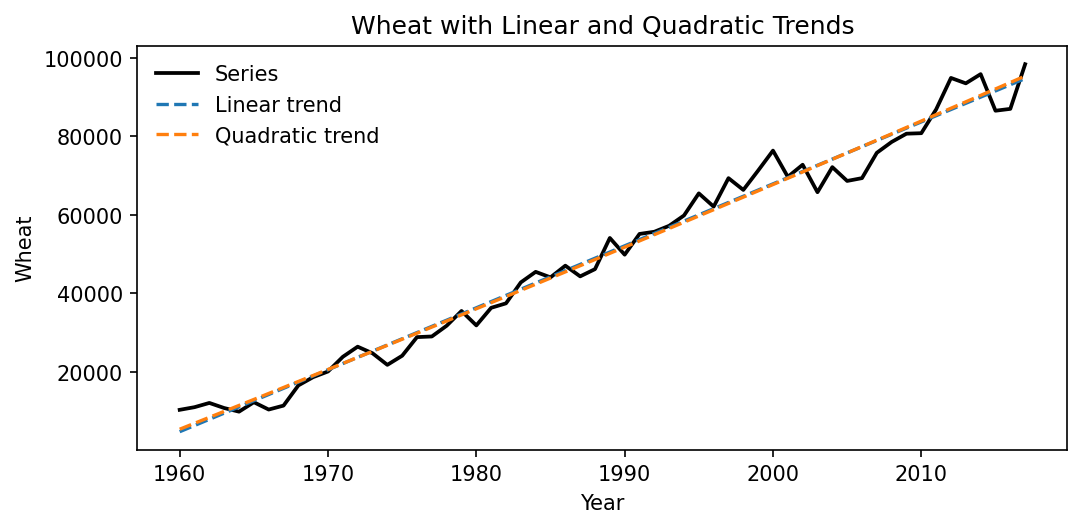
\includegraphics[width=0.95\linewidth]{S7.3B_wheat_trends.png}
\caption{Wheat series with linear and quadratic trend fits (dashed)}
\end{figure}
AIC: linear=1123.420, quadratic=1125.051; BIC: linear=1127.541, quadratic=1131.232. 
AIC and BIC both prefer the linear trend. This makes intuitive sense because the quadratic term is small and 
adds little visible curvature; information criteria penalize the extra parameter when the fit gain is minimal.
\end{document}